\documentclass[12pt]{article}
\usepackage[danish]{babel}
\usepackage{amsfonts, amssymb, mathtools, amsthm, amsmath}
\usepackage{graphicx, pgfplots}
\usepackage{url}
\usepackage[dvipsnames]{xcolor}
\usepackage{sagetex}
\usepackage{lastpage}

%loaded last
\usepackage[hidelinks]{hyperref}

\usepackage{siunitx}
  \sisetup{exponent-product = \cdot,
    output-decimal-marker = {,}}

%Giles Castelles incfig
\usepackage{import}
\usepackage{xifthen}
\usepackage{pdfpages}
\usepackage{transparent}

\newcommand{\incfig}[2][1]{%
  \def\svgwidth{#1\columnwidth}
  \import{../figures/}{#2.pdf_tex}
}

\setlength{\parindent}{0in}
\setlength{\oddsidemargin}{0in}
\setlength{\textwidth}{6.5in}
\setlength{\textheight}{8.8in}
\setlength{\topmargin}{0in}
\setlength{\headheight}{18pt}

\usepackage{fancyhdr}
\pagestyle{fancy}

\fancyhead{}
\fancyfoot{}
\fancyfoot[R]{\thepage}
\fancyhead[C]{\leftmark}

\pgfplotsset{compat=newest}

\pgfplotsset{every axis/.append style={
  axis x line=middle,    % put the x axis in the middle
  axis y line=middle,    % put the y axis in the middle
  axis line style={<->,color=black}, % arrows on the axis
}}

\usepackage{thmtools}
\usepackage{tcolorbox}
  \tcbuselibrary{skins, breakable}
  \tcbset{
    space to upper=1em,
    space to lower=1em,
  }

\theoremstyle{definition}

\newtcolorbox[auto counter]{definition}[1][]{%
  breakable,
  colframe=ForestGreen,  %frame color
  colback=ForestGreen!5, %background color
  colbacktitle=ForestGreen!25, %background color for title
  coltitle=ForestGreen!70!black,  %title color
  fonttitle=\bfseries\sffamily, %title font
  left=1em,              %space on left side in box,
  enhanced,              %more options
  frame hidden,          %hide frame
  borderline west={2pt}{0pt}{ForestGreen},  %display left line
  title=Definition \thetcbcounter: #1,
}

\newtcolorbox{greenline}{%
  breakable,
  colframe=ForestGreen,  %frame color
  colback=white,          %remove background color
  left=1em,              %space on left side in box
  enhanced,              %more options
  frame hidden,          %hide frame
  borderline west={2pt}{0pt}{ForestGreen},  %display left line
}

\newtcolorbox[auto counter, number within=section]{eks}[1][]{%
  brekable,
  colframe=NavyBlue,  %frame color
  colback=NavyBlue!5, %background color
  colbacktitle=NavyBlue!25,    %background color for title
  coltitle=NavyBlue!70!black,  %title color
  fonttitle=\bfseries\sffamily, %title font
  left=1em,            %space on left side in box,
  enhanced,            %more options
  frame hidden,        %hide frame
  borderline west={2pt}{0pt}{NavyBlue},  %display left line
  title=Eksempel \thetcbcounter: #1
}

\newtcolorbox{blueline}{%
  breakable,
  colframe=NavyBlue,     %frame color
  colback=white,         %remove background
  left=1em,              %space on left side in box,
  enhanced,              %more options
  frame hidden,          %hide frame
  borderline west={2pt}{0pt}{NavyBlue},  %display left line
}

\newtcolorbox{teo}[1][]{%
  breakable,
  colframe=RawSienna,  %frame color
  colback=RawSienna!5, %background color
  colbacktitle=RawSienna!25,    %background color for title
  coltitle=RawSienna!70!black,  %title color
  fonttitle=\bfseries\sffamily, %title font
  left=1em,              %space on left side in box,
  enhanced,              %more options
  frame hidden,          %hide frame
  borderline west={2pt}{0pt}{RawSienna},  %display left line
  title=Teori: #1,
}

\newtcolorbox[auto counter, number within=section]{sæt}[1][]{%
  breakable,
  colframe=RawSienna,  %frame color
  colback=RawSienna!5, %background color
  colbacktitle=RawSienna!25,    %background color for title
  coltitle=RawSienna!70!black,  %title color
  fonttitle=\bfseries\sffamily, %title font
  left=1em,              %space on left side in box,
  enhanced,              %more options
  frame hidden,          %hide frame
  borderline west={2pt}{0pt}{RawSienna},  %display left line
  title=Sætning \thetcbcounter: #1,
  before lower={\textbf{Bevis:}\par\vspace{0.5em}},
  colbacklower=RawSienna!25,
}

\newtcolorbox{redline}{%
  breakable,
  colframe=RawSienna,  %frame color
  colback=white,       %Remove background color
  left=1em,            %space on left side in box,
  enhanced,            %more options
  frame hidden,        %hide frame
  borderline west={2pt}{0pt}{RawSienna},  %display left line
}

\newtcolorbox{for}[1][]{%
  breakable,
  colframe=NavyBlue,  %frame color
  colback=NavyBlue!5, %background color
  colbacktitle=NavyBlue!25,    %background color for title
  coltitle=NavyBlue!70!black,  %title color
  fonttitle=\bfseries\sffamily, %title font
  left=1em,              %space on left side in box,
  enhanced,              %more options
  frame hidden,          %hide frame
  borderline west={2pt}{0pt}{NavyBlue},  %display left line
  title=Forklaring #1,
}

\newtcolorbox{bem}{%
  breakable,
  colframe=NavyBlue,  %frame color
  colback=NavyBlue!5, %background color
  colbacktitle=NavyBlue!25,    %background color for title
  coltitle=NavyBlue!70!black,  %title color
  fonttitle=\bfseries\sffamily, %title font
  left=1em,              %space on left side in box,
  enhanced,              %more options
  frame hidden,          %hide frame
  borderline west={2pt}{0pt}{NavyBlue},  %display left line
  title=Bemærkning:,
}

\makeatother
\def\@lecture{}%
\newcommand{\lecture}[3]{
  \ifthenelse{\isempty{#3}}{%
    \def\@lecture{Lecture #1}%
  }{%
    \def\@lecture{Lecture #1: #3}%
  }%
  \subsection*{\makebox[\textwidth][l]{\@lecture \hfill \normalfont\small\textsf{#2}}}
}

\makeatletter

\newcommand{\opgave}[1]{%
 \def\@opgave{#1}%
 \subsection*{Opgave #1}
}

\makeatother

%Format lim the same way in intext and in display
\let\svlim\lim\def\lim{\svlim\limits}

% horizontal rule
\newcommand\hr{
\noindent\rule[0.5ex]{\linewidth}{0.5pt}
}

\title{Opgaver til forelæsning uge 24}
\author{Noah Rahbek Bigum Hansen}
\date{27. November 2024}

\begin{document}

\maketitle

\section*{Opg. 12.45}
A sealed tank containing seawater to a height of \qty{11,0}{m} also contains air above the water at a gauge pressure of \qty{3,00}{atm}. Water flows out from the bottom through a small hole. How fast is this water moving?
\bigbreak
Vi har Bernoullis ligning for situationen som
\[ 
p_1 + \rho g y_1 +\frac{1}{2}\rho v_1^2 = p_2 + 0 + \frac{1}{2}\rho v_2^2
.\]
Fra kontinuitetsligningen har vi
\[ 
A_1 v_1 = A_2 v_2
.\]
Så idet det antages, at $A_1 \ll A_2$ fås, at $v_1 \approx 0$. Altså har vi
\[ 
p_1 + \rho \cdot g \cdot y_1 = p_2 + \frac{1}{2}\rho v_2^2
.\]
Idet $p = \qty{3,00}{atm}$ er et såkaldt \textit{gauge pressure} betyder det at $p_1$ er \qty{3,00}{atm} større end $p_2$ og vi får da
\begin{align*}
  \frac{1}{2}\rho v_2^2 &= p + \rho g y_1 \\
  v_2^2 &= \frac{2}{\rho} p + 2g y_1  \\
  v_2 &= \sqrt{\frac{2}{\rho} p + 2 g y_1} \\
  &= \sqrt{2 \frac{\qty{3,03975e5}{Pa}}{\qty{1000}{\frac{kg}{m^3}}} + 2 \cdot \qty{9,80}{\frac{m}{s^2}} \cdot \qty{11,0}{m}} \\
  &= \qty{28,7}{\frac{m}{s}} 
.\end{align*}




\section*{Opg. 12.51}
A golf course sprinkler system discharges water from a horizontal pipe at the rate of $\qty{7200}{\frac{cm^3}{s}}$. At one point in the pipe, where the radius is \qty{4,00}{cm}, the water’s absolute pressure is \qty{2,40e5}{Pa}. At a second point in the pipe, the water passes through a constriction where the radius is \qty{2,00}{cm}. What is the water’s absolute pressure as it flows through this constriction?
\bigbreak
Først findes tværsnitsarealerne af de to punkter i røret som hhv.
\begin{align*}
  A_1 &= \pi \cdot (\qty{4,00}{cm})^2 = \qty{50,27}{cm^2} \\
  A_2 &= \pi \cdot (\qty{2,00}{cm})^2 = \qty{12,57}{cm^2} 
.\end{align*}
Fra kontinuitetsligningen har vi desuden at
\[ 
  \qty{7200}{\frac{cm^3}{s}} = \frac{\mathrm{d}V}{\mathrm{d}t} = A_1v_1 = A_2v_2 
.\]
De to hastigheder kan da findes som
\begin{align*}
  v_1 &= \frac{1}{A_1} \frac{\mathrm{d}V}{\mathrm{d}t} = \frac{1}{\qty{50,72}{cm^2}} \cdot \qty{7200}{\frac{cm^3}{s}} = \qty{1,432}{\frac{m}{s}} \\
  v_2 &= \frac{1}{A_2} \frac{\mathrm{d}V}{\mathrm{d}t} = \frac{1}{\qty{12,57}{cm^2}} \cdot \qty{7200}{\frac{cm^3}{s}} = \qty{5,730}{\frac{m}{s}} 
.\end{align*}
Vi kan da benytte Bernoullis ligning til at finde trykket ved indsnævringen som
\begin{align*}
  p_1 + \frac{1}{2} \rho v_1^2 &= p_2 + \frac{1}{2} \rho v_2^2  \\
  p_2           &= p_1 + \frac{1}{2}\rho \left( v_1^2 - v_2^2 \right) \\
               &= \qty{2,40e5}{Pa} + \frac{\qty{1000}{\frac{kg}{m^3}}}{2} \left( \left( \qty{1,432}{\frac{m}{s}} \right)^2 - \left( \qty{5,730}{\frac{m}{s}}  \right)^2  \right) \\
               &= \qty{2,25e5}{Pa} 
.\end{align*}



\section*{Opg. 12.73}
A closed and elevated vertical cylindrical tank with diameter \qty{2,00}{m} contains water to a depth of \qty{0,800}{m}. A worker accidently pokes a circular hole with diameter \qty{0,0200}{m} in the bottom of the tank. As the water drains from the tank, compressed air above the water in the tank maintains a gauge pressure of \qty{5,00e3}{Pa} at the surface of the water. Ignore any effects of viscosity.

\subsection*{(a)}
Just after the hole is made, what is the speed of the water as it emerges from the hole? What is the ratio of this speed to the efflux speed if the top of the tank is open to the air?
\bigbreak
Idet vi har opgivet et \textit{gauge pressure} udgår det atmosfæriske tryk fra Bernoullis ligning så vi får, at
\[ 
p_1 + \rho g y_1 + \frac{1}{2}\rho v_1^2 = \frac{1}{2}\rho v_2^2
.\]
Vi har desuden kontinuitetsligningen, der siger, at
\[ 
  A_1 v_1 = A_2 v_2 \implies d_1^2 v_1 = d_2^2 v_2 \implies v_1 = \left( \frac{d_2}{d_1} \right)^2 v_2
.\]
Vi kan sætte dette ind i Bernoullis ligning som
\begin{align*}
  \frac{1}{2}\rho \left( v_2^2 - v_1^2 \right) &= p_1 + \rho g y_1 \\
  \frac{1}{2}\rho \left( v_2^2 - \left( \frac{d_2^2}{d_1^2} \right)^2 v_2^2 \right) &= p_1 + \rho g y_1  \\
  \frac{1}{2}\rho \left( 1 - \left( \frac{d_2}{d_1} \right)^2 \right) v_2^2 &= p_1 + \rho g y_1 \\
  v_2 &= \sqrt{\frac{2}{\rho \cdot \left( 1 - \left( \frac{d_2}{d_1} \right)^{4} \right)} (p_1 + \rho g y_1) }
.\end{align*}
Sættes tallene fra opgaven ind fås, at
\[ 
v_2 = \sqrt{\frac{2}{\qty{1000}{\frac{kg}{m^3}}  \left( 1 - \left( \frac{\qty{0,0200}{m}}{\qty{2,00}{m}} \right)^{4} \right)} (\qty{5,00e3}{Pa} + \qty{1000}{\frac{kg}{m^3}} \cdot \qty{9,80}{\frac{m}{s^2}} \cdot \qty{0,800}{m})} = \qty{5,07}{\frac{m}{s}} 
.\]
Altså er hastigheden på vandet der fosser ud netop i det der laves hul \qty{5,07}{m/s}.  

Samme beregning kan nu laves uden bidraget fra overtrykket på \qty{5,00e3}{Pa} indeni beholderen for at finde hastigheden, hvis der ikke var tryk i beholderen som
\[ 
  v_{2_a} = \sqrt{\frac{2 \cdot \qty{9,80}{\frac{m}{s^2}} \cdot \qty{0,800}{m} }{ 1 - \left( \frac{\qty{0,0200}{m} }{\qty{2,00}{m} } \right)^{4} }} = \qty{3,96}{\frac{m}{s}} 
.\]
Altså bliver forholdet
\[ 
\frac{\qty{5,07}{\frac{m}{s}}}{\qty{3,96}{\frac{m}{s}}} = \num{1,28} 
.\]



\subsection*{(b)}
How much time does it take for all the water to drain from the tank? What is the ratio of this time to the time it takes for the tank to drain if the top of the tank is open to the air?
\bigbreak
Vi har at $v_1 = - \frac{\mathrm{d}y}{\mathrm{d}t}$, da hastigheden af vandet i toppen af cylinderen nødvendigvis må tilsvare hastigheden som vandspejlet falder med. I (a) fandt vi et andet udtryk for $v_1$ og de to udtryk kan nu sættes lig hinanden som
\[ 
  v_1 = - \frac{\mathrm{d}y}{\mathrm{d}t} = \left( \frac{d_2}{d_1} \right)^2 v_2
.\]
Vi kan nu sætte dette ind i formlen for $v_2$ fra (a) som
\[ 
- \frac{\mathrm{d}y}{\mathrm{d}t} = \left( \frac{d_2}{d_1} \right)^2 \sqrt{\frac{2(p_1 + \rho g y_1)}{\rho \left( 1- \left( \frac{d_2}{d_1} \right)^{4} \right)}} 
.\]
Vi kan nu bemærke, at
\[ 
\frac{1}{1 - \left( \frac{d_2}{d_1} \right)^{4}} = \num{1,00000001} \approx 1 
.\]
Denne faktor ignoreres derfor i det følgende. Vi får da at
\[ 
- \frac{\mathrm{d}y}{\mathrm{d}t} = \left( \frac{d_2}{d_1} \right)^2 \sqrt{\frac{2}{\rho} \cdot (p_1 + \rho g y_1)}
.\]
Dette simplificerer til
\[ 
- \frac{\mathrm{d}y}{\mathrm{d}t} = \left( \frac{d_2}{d_1} \right)^2 \sqrt{2} \cdot \sqrt{ \frac{p_1 + \rho g y_1}{\rho}} = \left( \frac{d_2}{d_1} \right)^2 \sqrt{2g} \cdot \sqrt{\frac{p_1}{\rho g} + y_1}
.\]
Vi får altså at
\[ 
\frac{1}{\sqrt{\frac{p_1}{\rho g} + y}} \, \mathrm{d}\left( y + \frac{p_1}{\rho g} \right) = - \left( \frac{d_2}{d_1} \right)^2 \sqrt{2g} \, \mathrm{d}t 
.\]
Integralerne løses som
\begin{align*}
  \int_{y_1}^{0} \frac{1}{\sqrt{y + \frac{p_1}{\rho g}}} \, \mathrm{d} \left( y + \frac{p_1}{\rho g} \right) = - \left( \frac{d_2}{d_1} \right)^2 \sqrt{2g} \int_{0}^{t} \, \mathrm{d}t
.\end{align*}
Vi får da
\[ 
2 \sqrt{y + \frac{p_1}{\rho g}}  \bigg|_{y_1}^0 = - \left( \frac{d_2}{d_1} \right)^2 \sqrt{2g} t
.\]
Hvilket løses som
\begin{align*}
  2 \left( \sqrt{y_1 + \frac{p_1}{\rho g}} - \sqrt{\frac{p_1}{\rho g}} \, \right) &= \left( \frac{d_2}{d_1} \right)^2 \sqrt{2g}t \\
  t &= \frac{2}{\sqrt{2g}} \cdot \left( \frac{d_1}{d_2} \right)^2 \left( \sqrt{y_1 + \frac{p_1}{\rho g}} - \sqrt{\frac{p_1}{\rho g}} \, \right) \\
    &= \qty{1944}{s} = \qty{32,4}{min} = \qty{0,540}{hr} 
.\end{align*}

Sættes overtrykket i beholderen til 0 fås i stedet
\[ 
t = \qty{4041}{s}
.\]
Forholdet er altså
\[ 
\frac{\qty{4041}{s}}{\qty{1944}{s}} = \num{2,08} 
.\]




\section*{Opg. 12.80}
A cylindrical bucket, open at the top, is \qty{25,0}{cm} high and \qty{10,0}{cm} in diameter. A circular hole with a cross-sectional area \qty{1,50}{cm^2} is cut in the center of the bottom of the bucket. Water flows into the bucket from a tube above it at the rate of \qty{2,40e-4}{m^3/s} . How high will the water in the bucket rise?
\bigbreak
Vi har i opgaven fået oplyst, at
\[ 
\frac{\mathrm{d}V}{\mathrm{d}t} = \qty{2,40e-4}{\frac{m^3}{s}} 
.\]
Vi betragter nu tilfældet efter at vandniveuaet har stabiliseret sig. Her har vi 
\[ 
\frac{\mathrm{d}V}{\mathrm{d}t} = A_2 v_2
.\]
Vi kan altså finde udstrømningshastigheden som
\[ 
v_2 = \frac{\frac{\mathrm{d}V}{\mathrm{d}t} }{A_2} = \frac{\qty{2,4e-4}{m^\frac{3}{s}}}{\qty{1,50}{cm^2}} = \qty{1,60}{\frac{m}{s}} 
.\]
Vha. Bernoullis ligning kan der nu opstilles et udtryk for ``starthøjden'' af væsken som
\begin{align*}
  \rho g h &= \frac{1}{2}\rho v_2^2 \\
  h &= \frac{v_2^2}{2g} \\
    &= \frac{ \left( \qty{1,60}{\frac{m}{s^2}}  \right)^2 }{2 \cdot \qty{9,80}{\frac{m}{s^2}} }
    &= \qty{0,131}{m} = \qty{13,1}{cm} 
.\end{align*}



\section*{Opg. 12.83}
\begin{figure} [ht]
  \centering
  \caption{}
  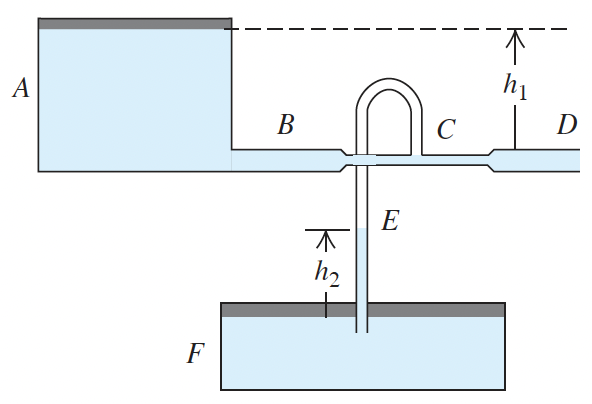
\includegraphics[width=0.3\linewidth]{../figures/F24_12_83.png}
  \label{fig:F24_12_83}
\end{figure}
Two very large open tanks $A$ and $F$ (\textbf{\autoref{fig:F24_12_83}}) contain the same liquid. A horizontal pipe $BCD$, having a constriction at $C$ and open to the air at $D$, leads out of the bottom of tank $A$, and a vertical pipe $E$ opens into the constriction at $C$ and dips into the liquid in tank $F$. Assume streamline flow and no viscosity. If the cross-sectional area at $C$ is one-half the area at $D$ and if $D$ is a distance $h_1$ below the level of the liquid in $A$, to what height $h_2$ will liquid rise in pipe $E$? Express your answer in terms of $h_1$.

\end{document}
